\begin{appendix}
\renewcommand{\thesection}{\bf 附錄 \Alph{section}}%設定標題名稱
\begin{center}
\fontsize{20pt}{0em}\selectfont\bf 附錄
\end{center}
\section*{LaTeX}
LaTex 為一種程式語言,支援標準庫 (Standard Libraries) 和外部程式庫 (External Libraries),不過與一般程式語言不同的是,它可以直接表述 Tex 排版結構,類似於 PHP 之於 HTML 的概念。但是直接撰寫 LaTex 仍較複雜,因此可以藉由 Markdown 這種輕量的標註式語言先行完成文章,再交由 LaTex 排版。
此專題報告採用編輯軟體為LaTeX,綜合對比Word編輯方法,LaTeX較為精準正確、更改、製作公式等,以便符合規範、製作。
 \begin{table}[htbp] %htbp代表表格浮動位置
			\centering%表格居中
			\caption{文字編輯軟體比較表}%表:標題
			\large%字體大小
			\label{tab_文字編輯軟體比較表:scale}
			\begin{tabular}{|c|c|c|c|c|c|c|}
			\hline
			\diagbox[width=5em]& 相容性 & 直觀性 & 文件排版 & 數學公式 & 微調細部\\ 
			\hline
			LaTeX 		&$\surd$&		&$\surd$&$\surd$&$\surd$\\
			\hline
			Word	 	&		&$\surd$&		&		&$\surd$\\
			\hline
			
			\end{tabular}
		\end{table}	

\begin{itemize} 
\item 特點:
\end{itemize}
\begin{enumerate}
\item 相容性:以Word為例會有版本差異,使用較高版本編輯的文件可能無法以較低的版本開啟,且不同作業系統也有些許差異;相比LaTeX可以利用不同編譯器進行編譯,且為免費軟體也可移植至可攜系統內,可以搭配Github協同編譯。
\item 文件排版:許多規範都會要求使用特定版型,使用文字編譯環境較能準確符合規定之版型,且能夠大範圍的自定義排定所需格式,並能不受之後更改而整體格式變形。
\item 數學公式呈現:LaTex可以直接利用本身多元的模組套件加入、編輯數學公式,在數學推導過程能夠快速的輸入自己需要的內容即可。
\item 細部調整:在大型論文、報告中有多項文字、圖片、表格,需要調整細部時,要在好幾頁中找尋,而LaTeX可以分段章節進行編譯,再進行合併處理大章節。
\end{enumerate}
\begin{figure}[hbt!]
\begin{center}
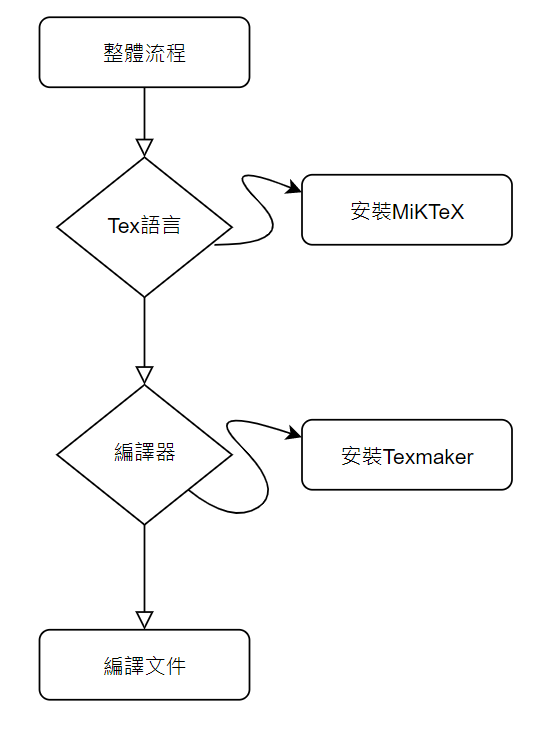
\includegraphics[width=10cm]{編譯流程}
\caption{\Large 編譯流程}
\label{fig.編譯流程}
\end{center}
\end{figure}
\end{appendix}
\section*{FFmpeg}
FFmpeg是一個開放原始碼的自由軟體,可以對音訊和視訊進行多種格式的錄影、轉檔、串流功能。在專題訓練過程中透過FFmpeg的視訊錄製的功能記錄對打影像來了解實際訓練狀況。
\newpage